\documentclass[11pt,]{article}
\usepackage{lmodern}
\usepackage{amssymb,amsmath}
\usepackage{ifxetex,ifluatex}
\usepackage{fixltx2e} % provides \textsubscript
\ifnum 0\ifxetex 1\fi\ifluatex 1\fi=0 % if pdftex
  \usepackage[T1]{fontenc}
  \usepackage[utf8]{inputenc}
\else % if luatex or xelatex
  \ifxetex
    \usepackage{mathspec}
  \else
    \usepackage{fontspec}
  \fi
  \defaultfontfeatures{Ligatures=TeX,Scale=MatchLowercase}
\fi
% use upquote if available, for straight quotes in verbatim environments
\IfFileExists{upquote.sty}{\usepackage{upquote}}{}
% use microtype if available
\IfFileExists{microtype.sty}{%
\usepackage{microtype}
\UseMicrotypeSet[protrusion]{basicmath} % disable protrusion for tt fonts
}{}
\usepackage[margin=.75in]{geometry}
\usepackage{hyperref}
\hypersetup{unicode=true,
            pdftitle={Problem Set \#5},
            pdfauthor={Anaya Hall and Christian Miller},
            pdfborder={0 0 0},
            breaklinks=true}
\urlstyle{same}  % don't use monospace font for urls
\usepackage{color}
\usepackage{fancyvrb}
\newcommand{\VerbBar}{|}
\newcommand{\VERB}{\Verb[commandchars=\\\{\}]}
\DefineVerbatimEnvironment{Highlighting}{Verbatim}{commandchars=\\\{\}}
% Add ',fontsize=\small' for more characters per line
\usepackage{framed}
\definecolor{shadecolor}{RGB}{248,248,248}
\newenvironment{Shaded}{\begin{snugshade}}{\end{snugshade}}
\newcommand{\KeywordTok}[1]{\textcolor[rgb]{0.13,0.29,0.53}{\textbf{#1}}}
\newcommand{\DataTypeTok}[1]{\textcolor[rgb]{0.13,0.29,0.53}{#1}}
\newcommand{\DecValTok}[1]{\textcolor[rgb]{0.00,0.00,0.81}{#1}}
\newcommand{\BaseNTok}[1]{\textcolor[rgb]{0.00,0.00,0.81}{#1}}
\newcommand{\FloatTok}[1]{\textcolor[rgb]{0.00,0.00,0.81}{#1}}
\newcommand{\ConstantTok}[1]{\textcolor[rgb]{0.00,0.00,0.00}{#1}}
\newcommand{\CharTok}[1]{\textcolor[rgb]{0.31,0.60,0.02}{#1}}
\newcommand{\SpecialCharTok}[1]{\textcolor[rgb]{0.00,0.00,0.00}{#1}}
\newcommand{\StringTok}[1]{\textcolor[rgb]{0.31,0.60,0.02}{#1}}
\newcommand{\VerbatimStringTok}[1]{\textcolor[rgb]{0.31,0.60,0.02}{#1}}
\newcommand{\SpecialStringTok}[1]{\textcolor[rgb]{0.31,0.60,0.02}{#1}}
\newcommand{\ImportTok}[1]{#1}
\newcommand{\CommentTok}[1]{\textcolor[rgb]{0.56,0.35,0.01}{\textit{#1}}}
\newcommand{\DocumentationTok}[1]{\textcolor[rgb]{0.56,0.35,0.01}{\textbf{\textit{#1}}}}
\newcommand{\AnnotationTok}[1]{\textcolor[rgb]{0.56,0.35,0.01}{\textbf{\textit{#1}}}}
\newcommand{\CommentVarTok}[1]{\textcolor[rgb]{0.56,0.35,0.01}{\textbf{\textit{#1}}}}
\newcommand{\OtherTok}[1]{\textcolor[rgb]{0.56,0.35,0.01}{#1}}
\newcommand{\FunctionTok}[1]{\textcolor[rgb]{0.00,0.00,0.00}{#1}}
\newcommand{\VariableTok}[1]{\textcolor[rgb]{0.00,0.00,0.00}{#1}}
\newcommand{\ControlFlowTok}[1]{\textcolor[rgb]{0.13,0.29,0.53}{\textbf{#1}}}
\newcommand{\OperatorTok}[1]{\textcolor[rgb]{0.81,0.36,0.00}{\textbf{#1}}}
\newcommand{\BuiltInTok}[1]{#1}
\newcommand{\ExtensionTok}[1]{#1}
\newcommand{\PreprocessorTok}[1]{\textcolor[rgb]{0.56,0.35,0.01}{\textit{#1}}}
\newcommand{\AttributeTok}[1]{\textcolor[rgb]{0.77,0.63,0.00}{#1}}
\newcommand{\RegionMarkerTok}[1]{#1}
\newcommand{\InformationTok}[1]{\textcolor[rgb]{0.56,0.35,0.01}{\textbf{\textit{#1}}}}
\newcommand{\WarningTok}[1]{\textcolor[rgb]{0.56,0.35,0.01}{\textbf{\textit{#1}}}}
\newcommand{\AlertTok}[1]{\textcolor[rgb]{0.94,0.16,0.16}{#1}}
\newcommand{\ErrorTok}[1]{\textcolor[rgb]{0.64,0.00,0.00}{\textbf{#1}}}
\newcommand{\NormalTok}[1]{#1}
\usepackage{longtable,booktabs}
\usepackage{graphicx,grffile}
\makeatletter
\def\maxwidth{\ifdim\Gin@nat@width>\linewidth\linewidth\else\Gin@nat@width\fi}
\def\maxheight{\ifdim\Gin@nat@height>\textheight\textheight\else\Gin@nat@height\fi}
\makeatother
% Scale images if necessary, so that they will not overflow the page
% margins by default, and it is still possible to overwrite the defaults
% using explicit options in \includegraphics[width, height, ...]{}
\setkeys{Gin}{width=\maxwidth,height=\maxheight,keepaspectratio}
\IfFileExists{parskip.sty}{%
\usepackage{parskip}
}{% else
\setlength{\parindent}{0pt}
\setlength{\parskip}{6pt plus 2pt minus 1pt}
}
\setlength{\emergencystretch}{3em}  % prevent overfull lines
\providecommand{\tightlist}{%
  \setlength{\itemsep}{0pt}\setlength{\parskip}{0pt}}
\setcounter{secnumdepth}{0}
% Redefines (sub)paragraphs to behave more like sections
\ifx\paragraph\undefined\else
\let\oldparagraph\paragraph
\renewcommand{\paragraph}[1]{\oldparagraph{#1}\mbox{}}
\fi
\ifx\subparagraph\undefined\else
\let\oldsubparagraph\subparagraph
\renewcommand{\subparagraph}[1]{\oldsubparagraph{#1}\mbox{}}
\fi

%%% Use protect on footnotes to avoid problems with footnotes in titles
\let\rmarkdownfootnote\footnote%
\def\footnote{\protect\rmarkdownfootnote}

%%% Change title format to be more compact
\usepackage{titling}

% Create subtitle command for use in maketitle
\newcommand{\subtitle}[1]{
  \posttitle{
    \begin{center}\large#1\end{center}
    }
}

\setlength{\droptitle}{-2em}
  \title{Problem Set \#5}
  \pretitle{\vspace{\droptitle}\centering\huge}
  \posttitle{\par}
  \author{Anaya Hall and Christian Miller}
  \preauthor{\centering\large\emph}
  \postauthor{\par}
  \predate{\centering\large\emph}
  \postdate{\par}
  \date{5/2/2018}

\usepackage{booktabs}
\usepackage{longtable}
\usepackage{array}
\usepackage{multirow}
\usepackage[table]{xcolor}
\usepackage{wrapfig}
\usepackage{float}
\usepackage{colortbl}
\usepackage{pdflscape}
\usepackage{tabu}
\usepackage{threeparttable}
\usepackage[normalem]{ulem}

\begin{document}
\maketitle

\section{Part 1: Theory}\label{part-1-theory}

(Optional -- skip for now!)

\section{Part 2: Instrumental
Variables}\label{part-2-instrumental-variables}

\subsection{Question 1: NLS80}\label{question-1-nls80}

Revisit the model from \emph{Problem Set \#3}, now including ability.

\(log(wage) = \beta_0 + exper \cdot \beta_1 + tenure \cdot \beta_2 + married \cdot \beta_3 + south \cdot \beta_4 + urban \cdot \beta_5 + black \cdot \beta_6 + educ \cdot \beta_7 + abil \cdot \gamma + \epsilon\)

\begin{Shaded}
\begin{Highlighting}[]
\CommentTok{# Read in CSV as data.frame}
\NormalTok{wage_df <-}\StringTok{ }\NormalTok{readr}\OperatorTok{::}\KeywordTok{read_csv}\NormalTok{(}\StringTok{"nls80.csv"}\NormalTok{)}

\CommentTok{# Select only the variables in our model}
\NormalTok{wage_df }\OperatorTok\StringTok{ }\KeywordTok{select}\NormalTok{(lwage, wage, exper, tenure, married, south, urban, black, educ, iq)}
\end{Highlighting}
\end{Shaded}

\subsubsection{(a) Bias of coefficient on
education}\label{a-bias-of-coefficient-on-education}

Derive the bias of \(\beta_7\). Show which direction the bias goes in
depending on whether the correlation between ability and education is
positive or negative.

\$ abil = \delta\_0 + exper \cdot \delta\_1 + tenure \cdot \delta\_2 +
married \cdot \delta\_3 + south \cdot \delta\_4 + urban \cdot \delta\_5
+ black \cdot \delta\_6 + educ \cdot \delta\_7 + \eta\$

\(log(wage) = (\beta_0 + \gamma \delta_0) + exper \cdot (\beta_1 + \gamma \delta_1) + tenure \cdot (\beta_2 + \gamma \delta_2) + married \cdot (\beta_3 + \gamma \delta_3) + south \cdot (\beta_4 + \gamma \delta_4) + urban \cdot (\beta_5 + \gamma \delta_5) + black \cdot (\beta_6 + \gamma \delta_6) + educ \cdot (\beta_7 + \gamma \delta_7) + \gamma \eta + v\)

Assume that all \(\delta\)'s are zero except for the one on the variable
of interest (education)

\(log(wage) = \beta_0 + exper \cdot \beta_1 + tenure \cdot \beta_2 + married \cdot \beta_3 + south \cdot \beta_4 + urban \cdot \beta_5 + black \cdot \beta_6 + educ \cdot (\beta_7 + \gamma \delta_7) + \gamma \eta + v\)

Where

\(plim b_7 = \beta_7 + \gamma \delta_7\)

\(plim b_7 = \beta_7 + \gamma \cdot \frac {Cov [ abil , educ ]} {Var [educ]}\)

Truth is \(\beta_7\) , bias is
\(\gamma \cdot \frac {Cov [ abil , educ ]} {Var [educ]}\)

We expect the sign on \(\gamma\) to be positive (higher abiltiy should
lead to higher wage), the covariance of ability and education to also be
positive (more able people acheive higher levels of education), and, of
course, the variance of education is positive. Thus, the bias will also
be \emph{positive} (biased upward! i.e.~we will over attribute the
effect of education on wage).

\subsubsection{(b) Proxy for ability}\label{b-proxy-for-ability}

Estimate the model above excluding ability, record your parameter
estimates, standard errors and \(R^2\).

\subparagraph{- OLS function -}\label{ols-function--}

First, let's load our OLS function.

\begin{Shaded}
\begin{Highlighting}[]
\CommentTok{# Function to convert tibble, data.frame, or tbl_df to matrix}
\NormalTok{to_matrix <-}\StringTok{ }\ControlFlowTok{function}\NormalTok{(the_df, vars) \{}
  \CommentTok{# Create a matrix from variables in var}
\NormalTok{  new_mat <-}\StringTok{ }\NormalTok{the_df }\OperatorTok
\StringTok{    }\CommentTok{#Select the columns given in 'vars'}
\StringTok{    }\KeywordTok{select_}\NormalTok{(}\DataTypeTok{.dots =}\NormalTok{ vars) }\OperatorTok
\StringTok{    }\CommentTok{# Convert to matrix}
\StringTok{    }\KeywordTok{as.matrix}\NormalTok{()}
  \CommentTok{# Return 'new_mat'}
  \KeywordTok{return}\NormalTok{(new_mat)}
\NormalTok{\}}


\NormalTok{b_ols <-}\StringTok{ }\ControlFlowTok{function}\NormalTok{(y, X) \{}
  \CommentTok{# Calculate beta hat}
\NormalTok{  beta_hat <-}\StringTok{ }\KeywordTok{solve}\NormalTok{(}\KeywordTok{t}\NormalTok{(X) }\OperatorTok\StringTok{ }\NormalTok{X) }\OperatorTok\StringTok{ }\KeywordTok{t}\NormalTok{(X) }\OperatorTok\StringTok{ }\NormalTok{y}
  \CommentTok{# Return beta_hat}
  \KeywordTok{return}\NormalTok{(beta_hat)}
\NormalTok{\}}

\NormalTok{ols <-}\StringTok{ }\ControlFlowTok{function}\NormalTok{(data, y_data, X_data, }\DataTypeTok{intercept =}\NormalTok{ T, }\DataTypeTok{hetsked =}\NormalTok{ F, }\DataTypeTok{H0 =} \DecValTok{0}\NormalTok{, }\DataTypeTok{two_tail =}\NormalTok{ T, }\DataTypeTok{alpha =} \FloatTok{0.05}\NormalTok{) \{}
  \CommentTok{# Function setup ----}
    \CommentTok{# Require the 'dplyr' package}
    \KeywordTok{require}\NormalTok{(dplyr)}
  
  \CommentTok{# Create dependent and independent variable matrices ----}
    \CommentTok{# y matrix}
\NormalTok{    y <-}\StringTok{ }\KeywordTok{to_matrix}\NormalTok{ (}\DataTypeTok{the_df =}\NormalTok{ data, }\DataTypeTok{vars =}\NormalTok{ y_data)}
    \CommentTok{# X matrix}
\NormalTok{    X <-}\StringTok{ }\KeywordTok{to_matrix}\NormalTok{ (}\DataTypeTok{the_df =}\NormalTok{ data, }\DataTypeTok{vars =}\NormalTok{ X_data)}
      \CommentTok{# If 'intercept' is TRUE, then add a column of ones}
      \ControlFlowTok{if}\NormalTok{ (intercept }\OperatorTok{==}\StringTok{ }\NormalTok{T) \{}
\NormalTok{      X <-}\StringTok{ }\KeywordTok{cbind}\NormalTok{(}\DecValTok{1}\NormalTok{,X)}
      \KeywordTok{colnames}\NormalTok{(X) <-}\StringTok{ }\KeywordTok{c}\NormalTok{(}\StringTok{"intercept"}\NormalTok{, X_data)}
\NormalTok{      \}}
 
  \CommentTok{# Calculate b, y_hat, and residuals ----}
\NormalTok{    b <-}\StringTok{ }\KeywordTok{solve}\NormalTok{(}\KeywordTok{t}\NormalTok{(X) }\OperatorTok\StringTok{ }\NormalTok{X) }\OperatorTok\StringTok{ }\KeywordTok{t}\NormalTok{(X) }\OperatorTok\StringTok{ }\NormalTok{y}
\NormalTok{    y_hat <-}\StringTok{ }\NormalTok{X }\OperatorTok\StringTok{ }\NormalTok{b}
\NormalTok{    e <-}\StringTok{ }\NormalTok{y }\OperatorTok{-}\StringTok{ }\NormalTok{y_hat}
   
    \CommentTok{# Inverse of X'X}
\NormalTok{    XX <-}\StringTok{ }\KeywordTok{t}\NormalTok{(X) }\OperatorTok\StringTok{ }\NormalTok{X}
\NormalTok{    XX_inv <-}\StringTok{ }\KeywordTok{solve}\NormalTok{(}\KeywordTok{t}\NormalTok{(X) }\OperatorTok\StringTok{ }\NormalTok{X)}
    
    \ControlFlowTok{if}\NormalTok{ (hetsked }\OperatorTok{==}\StringTok{ }\NormalTok{T) \{}
      \CommentTok{# For each row, calculate x_i' x_i e_i^2; then sum}
\NormalTok{     sigma_hat <-}\StringTok{ }\KeywordTok{lapply}\NormalTok{(}\DataTypeTok{X =} \DecValTok{1}\OperatorTok{:}\NormalTok{n, }\DataTypeTok{FUN =} \ControlFlowTok{function}\NormalTok{(i) \{}
      \CommentTok{# Define x_i}
\NormalTok{      x_i <-}\StringTok{ }\KeywordTok{matrix}\NormalTok{(}\KeywordTok{as.vector}\NormalTok{(X[i,]), }\DataTypeTok{nrow =} \DecValTok{1}\NormalTok{)}
      \CommentTok{# Return x_i' x_i e_i^2}
      \KeywordTok{return}\NormalTok{(}\KeywordTok{t}\NormalTok{(x_i) }\OperatorTok\StringTok{ }\NormalTok{x_i }\OperatorTok{*}\StringTok{ }\NormalTok{e[i]}\OperatorTok{^}\DecValTok{2}\NormalTok{)}
\NormalTok{      \}) }\OperatorTok\StringTok{ }\KeywordTok{Reduce}\NormalTok{(}\DataTypeTok{f =} \StringTok{"+"}\NormalTok{, }\DataTypeTok{x =}\NormalTok{ .) \}}
    
    \ControlFlowTok{if}\NormalTok{ (hetsked }\OperatorTok{==}\StringTok{ }\NormalTok{F) sigma_hat <-}\StringTok{ }\NormalTok{XX}
    
  \CommentTok{# Useful -----}
\NormalTok{    n <-}\StringTok{ }\KeywordTok{nrow}\NormalTok{(X) }\CommentTok{# number of observations}
\NormalTok{    k <-}\StringTok{ }\KeywordTok{ncol}\NormalTok{(X) }\CommentTok{# number of independent variables}
\NormalTok{    dof <-}\StringTok{ }\NormalTok{n }\OperatorTok{-}\StringTok{ }\NormalTok{k }\CommentTok{# degrees of freedom}
\NormalTok{    i <-}\StringTok{ }\KeywordTok{rep}\NormalTok{(}\DecValTok{1}\NormalTok{,n) }\CommentTok{# column of ones for demeaning matrix}
\NormalTok{    A <-}\StringTok{ }\KeywordTok{diag}\NormalTok{(i) }\OperatorTok{-}\StringTok{ }\NormalTok{(}\DecValTok{1} \OperatorTok{/}\StringTok{ }\NormalTok{n) }\OperatorTok{*}\StringTok{ }\NormalTok{i }\OperatorTok\StringTok{ }\KeywordTok{t}\NormalTok{(i) }\CommentTok{# demeaning matrix}
\NormalTok{    y_star <-}\StringTok{ }\NormalTok{A }\OperatorTok\StringTok{ }\NormalTok{y }\CommentTok{# for SST}
\NormalTok{    X_star <-}\StringTok{ }\NormalTok{A }\OperatorTok\StringTok{ }\NormalTok{X }\CommentTok{# for SSM}
\NormalTok{    SST <-}\StringTok{ }\KeywordTok{drop}\NormalTok{(}\KeywordTok{t}\NormalTok{(y_star) }\OperatorTok\StringTok{ }\NormalTok{y_star)}
\NormalTok{    SSM <-}\StringTok{ }\KeywordTok{drop}\NormalTok{(}\KeywordTok{t}\NormalTok{(b) }\OperatorTok\StringTok{ }\KeywordTok{t}\NormalTok{(X_star) }\OperatorTok\StringTok{ }\NormalTok{X_star }\OperatorTok\StringTok{ }\NormalTok{b)}
\NormalTok{    SSR <-}\StringTok{ }\KeywordTok{drop}\NormalTok{(}\KeywordTok{t}\NormalTok{(e) }\OperatorTok\StringTok{ }\NormalTok{e)}
  
  \CommentTok{# Measures of fit and estimated variance ----}
\NormalTok{    R2uc <-}\StringTok{ }\KeywordTok{drop}\NormalTok{((}\KeywordTok{t}\NormalTok{(y_hat) }\OperatorTok\StringTok{ }\NormalTok{y_hat)}\OperatorTok{/}\NormalTok{(}\KeywordTok{t}\NormalTok{(y) }\OperatorTok\StringTok{ }\NormalTok{y)) }\CommentTok{# Uncentered R^2}
\NormalTok{    R2 <-}\StringTok{ }\DecValTok{1} \OperatorTok{-}\StringTok{ }\NormalTok{SSR}\OperatorTok{/}\NormalTok{SST }\CommentTok{# Uncentered R^2}
\NormalTok{    R2adj <-}\StringTok{ }\DecValTok{1} \OperatorTok{-}\StringTok{ }\NormalTok{(n}\OperatorTok{-}\DecValTok{1}\NormalTok{)}\OperatorTok{/}\NormalTok{dof }\OperatorTok{*}\StringTok{ }\NormalTok{(}\DecValTok{1} \OperatorTok{-}\StringTok{ }\NormalTok{R2) }\CommentTok{# Adjusted R^2}
\NormalTok{    AIC <-}\StringTok{ }\KeywordTok{log}\NormalTok{(SSR}\OperatorTok{/}\NormalTok{n) }\OperatorTok{+}\StringTok{ }\DecValTok{2}\OperatorTok{*}\NormalTok{k}\OperatorTok{/}\NormalTok{n }\CommentTok{# AIC}
\NormalTok{    SIC <-}\StringTok{ }\KeywordTok{log}\NormalTok{(SSR}\OperatorTok{/}\NormalTok{n) }\OperatorTok{+}\StringTok{ }\NormalTok{k}\OperatorTok{/}\NormalTok{n}\OperatorTok{*}\KeywordTok{log}\NormalTok{(n) }\CommentTok{# SIC}
\NormalTok{    s2 <-}\StringTok{ }\NormalTok{SSR}\OperatorTok{/}\NormalTok{dof }\CommentTok{# s^2}
  
  \CommentTok{# Measures of fit table ----}
\NormalTok{    mof_table_df <-}\StringTok{ }\KeywordTok{data.frame}\NormalTok{(R2uc, R2, R2adj, SIC, AIC, SSR, s2)}
\NormalTok{    mof_table_col_names <-}\StringTok{ }\KeywordTok{c}\NormalTok{(}\StringTok{"$R^2_}\CharTok{\textbackslash{}\textbackslash{}}\StringTok{text\{uc\}$"}\NormalTok{, }\StringTok{"$R^2$"}\NormalTok{,}
                             \StringTok{"$R^2_}\CharTok{\textbackslash{}\textbackslash{}}\StringTok{text\{adj\}$"}\NormalTok{,}
                             \StringTok{"SIC"}\NormalTok{, }\StringTok{"AIC"}\NormalTok{, }\StringTok{"SSR"}\NormalTok{, }\StringTok{"$s^2$"}\NormalTok{)}
\NormalTok{    mof_table <-}\StringTok{  }\NormalTok{mof_table_df }\OperatorTok\StringTok{ }\NormalTok{knitr}\OperatorTok{::}\KeywordTok{kable}\NormalTok{(}
      \DataTypeTok{row.names =}\NormalTok{ F,}
      \DataTypeTok{col.names =}\NormalTok{ mof_table_col_names,}
      \DataTypeTok{format.args =} \KeywordTok{list}\NormalTok{(}\DataTypeTok{scientific =}\NormalTok{ F, }\DataTypeTok{digits =} \DecValTok{4}\NormalTok{),}
      \DataTypeTok{booktabs =}\NormalTok{ T,}
      \DataTypeTok{escape =}\NormalTok{ F}
\NormalTok{    )}
  
  \CommentTok{# t-test----}
    \CommentTok{# Standard error}
\NormalTok{    se <-}\StringTok{ }\KeywordTok{sqrt}\NormalTok{(s2 }\OperatorTok{*}\StringTok{ }\KeywordTok{diag}\NormalTok{(XX_inv }\OperatorTok\StringTok{ }\NormalTok{sigma_hat }\OperatorTok\StringTok{ }\NormalTok{XX_inv)) }\CommentTok{# Vector of _t_ statistics}
    \CommentTok{# Vector of _t_ statistics}
\NormalTok{    t_stats <-}\StringTok{ }\NormalTok{(b }\OperatorTok{-}\StringTok{ }\NormalTok{H0) }\OperatorTok{/}\StringTok{ }\NormalTok{se}
    \CommentTok{# Calculate the p-values}
    \ControlFlowTok{if}\NormalTok{ (two_tail }\OperatorTok{==}\StringTok{ }\NormalTok{T) \{}
\NormalTok{    p_values <-}\StringTok{ }\KeywordTok{pt}\NormalTok{(}\DataTypeTok{q =} \KeywordTok{abs}\NormalTok{(t_stats), }\DataTypeTok{df =}\NormalTok{ dof, }\DataTypeTok{lower.tail =}\NormalTok{ F) }\OperatorTok{*}\StringTok{ }\DecValTok{2}
\NormalTok{    \} }\ControlFlowTok{else}\NormalTok{ \{}
\NormalTok{      p_values <-}\StringTok{ }\KeywordTok{pt}\NormalTok{(}\DataTypeTok{q =} \KeywordTok{abs}\NormalTok{(t_stats), }\DataTypeTok{df =}\NormalTok{ dof, }\DataTypeTok{lower.tail =}\NormalTok{ F)}
\NormalTok{    \}}
    \CommentTok{# Do we (fail to) reject?}
\NormalTok{    reject <-}\StringTok{ }\KeywordTok{ifelse}\NormalTok{(p_values }\OperatorTok{<}\StringTok{ }\NormalTok{alpha, reject <-}\StringTok{ "Reject"}\NormalTok{, reject <-}\StringTok{ "Fail to Reject"}\NormalTok{)}
    
    \CommentTok{# Nice table (data.frame) of results}
\NormalTok{    ttest_df <-}\StringTok{ }\KeywordTok{data.frame}\NormalTok{(}
      \CommentTok{# The rows have the coef. names}
      \DataTypeTok{effect =} \KeywordTok{rownames}\NormalTok{(b),}
      \CommentTok{# Estimated coefficients}
      \DataTypeTok{coef =} \KeywordTok{as.vector}\NormalTok{(b) }\OperatorTok\StringTok{ }\KeywordTok{round}\NormalTok{(}\DecValTok{3}\NormalTok{),}
      \CommentTok{# Standard errors}
      \DataTypeTok{std_error =} \KeywordTok{as.vector}\NormalTok{(se) }\OperatorTok\StringTok{ }\KeywordTok{round}\NormalTok{(}\DecValTok{4}\NormalTok{),}
      \CommentTok{# t statistics}
      \DataTypeTok{t_stat =} \KeywordTok{as.vector}\NormalTok{(t_stats) }\OperatorTok\StringTok{ }\KeywordTok{round}\NormalTok{(}\DecValTok{3}\NormalTok{),}
      \CommentTok{# p-values}
      \DataTypeTok{p_value =} \KeywordTok{as.vector}\NormalTok{(p_values) }\OperatorTok\StringTok{ }\KeywordTok{round}\NormalTok{(}\DecValTok{4}\NormalTok{),}
      \CommentTok{# reject null?}
      \DataTypeTok{significance =} \KeywordTok{as.character}\NormalTok{(reject)}
\NormalTok{      )}
  
\NormalTok{    ttest_table <-}\StringTok{  }\NormalTok{ttest_df }\OperatorTok\StringTok{ }\NormalTok{knitr}\OperatorTok{::}\KeywordTok{kable}\NormalTok{(}
      \DataTypeTok{col.names =} \KeywordTok{c}\NormalTok{(}\StringTok{""}\NormalTok{, }\StringTok{"Coef."}\NormalTok{, }\StringTok{"S.E."}\NormalTok{, }\StringTok{"t Stat"}\NormalTok{, }\StringTok{"p-Value"}\NormalTok{, }\StringTok{"Decision"}\NormalTok{),}
      \DataTypeTok{booktabs =}\NormalTok{ T,}
      \DataTypeTok{format.args =} \KeywordTok{list}\NormalTok{(}\DataTypeTok{scientific =}\NormalTok{ F),}
      \DataTypeTok{escape =}\NormalTok{ F,}
      \DataTypeTok{caption =} \StringTok{"OLS Results"}
\NormalTok{    )}

  \CommentTok{# Data frame for exporting for y, y_hat, X, and e vectors ----}
\NormalTok{    export_df <-}\StringTok{ }\KeywordTok{data.frame}\NormalTok{(y, y_hat, e, X) }\OperatorTok\StringTok{ }\KeywordTok{tbl_df}\NormalTok{()}
    \KeywordTok{colnames}\NormalTok{(export_df) <-}\StringTok{ }\KeywordTok{c}\NormalTok{(}\StringTok{"y"}\NormalTok{,}\StringTok{"y_hat"}\NormalTok{,}\StringTok{"e"}\NormalTok{,}\KeywordTok{colnames}\NormalTok{(X))}
  
  \CommentTok{# Return ----}
    \KeywordTok{return}\NormalTok{(}\KeywordTok{list}\NormalTok{(}\DataTypeTok{n=}\NormalTok{n, }\DataTypeTok{dof=}\NormalTok{dof, }\DataTypeTok{b=}\NormalTok{b, }\DataTypeTok{se=}\NormalTok{se, }\DataTypeTok{vars=}\NormalTok{export_df, }\DataTypeTok{R2uc=}\NormalTok{R2uc,}\DataTypeTok{R2=}\NormalTok{R2,}
                \DataTypeTok{R2adj=}\NormalTok{R2adj, }\DataTypeTok{AIC=}\NormalTok{AIC, }\DataTypeTok{SIC=}\NormalTok{SIC, }\DataTypeTok{s2=}\NormalTok{s2, }\DataTypeTok{SST=}\NormalTok{SST, }\DataTypeTok{SSR=}\NormalTok{SSR,}
                \DataTypeTok{mof_table=}\NormalTok{mof_table, }\DataTypeTok{ttest=}\NormalTok{ttest_table))}
\NormalTok{\}}
\end{Highlighting}
\end{Shaded}

\newpage

\begin{Shaded}
\begin{Highlighting}[]
\NormalTok{model_}\DecValTok{1}\NormalTok{ <-}\StringTok{ }\KeywordTok{ols}\NormalTok{(wage_df, }\DataTypeTok{y_data =} \StringTok{"lwage"}\NormalTok{, }
               \DataTypeTok{X_data =} \KeywordTok{c}\NormalTok{(}\StringTok{"exper"}\NormalTok{, }\StringTok{"tenure"}\NormalTok{, }\StringTok{"married"}\NormalTok{, }\StringTok{"south"}\NormalTok{, }\StringTok{"urban"}\NormalTok{, }\StringTok{"black"}\NormalTok{, }\StringTok{"educ"}\NormalTok{))}

\NormalTok{model_}\DecValTok{1}\OperatorTok{$}\NormalTok{ttest}
\end{Highlighting}
\end{Shaded}

\begin{longtable}[]{@{}lrrrrl@{}}
\caption{OLS Results}\tabularnewline
\toprule
& Coef. & S.E. & t Stat & p-Value & Decision\tabularnewline
\midrule
\endfirsthead
\toprule
& Coef. & S.E. & t Stat & p-Value & Decision\tabularnewline
\midrule
\endhead
intercept & 5.395 & 0.1132 & 47.653 & 0.0000 & Reject\tabularnewline
exper & 0.014 & 0.0032 & 4.409 & 0.0000 & Reject\tabularnewline
tenure & 0.012 & 0.0025 & 4.789 & 0.0000 & Reject\tabularnewline
married & 0.199 & 0.0391 & 5.107 & 0.0000 & Reject\tabularnewline
south & -0.091 & 0.0262 & -3.463 & 0.0006 & Reject\tabularnewline
urban & 0.184 & 0.0270 & 6.822 & 0.0000 & Reject\tabularnewline
black & -0.188 & 0.0377 & -5.000 & 0.0000 & Reject\tabularnewline
educ & 0.065 & 0.0063 & 10.468 & 0.0000 & Reject\tabularnewline
\bottomrule
\end{longtable}

\begin{Shaded}
\begin{Highlighting}[]
\NormalTok{model_}\DecValTok{1}\OperatorTok{$}\NormalTok{mof}
\end{Highlighting}
\end{Shaded}

\begin{longtable}[]{@{}rrrrrrr@{}}
\toprule
\(R^2_\text{uc}\) & \(R^2\) & \(R^2_\text{adj}\) & SIC & AIC & SSR &
\(s^2\)\tabularnewline
\midrule
\endhead
0.9971 & 0.2526 & 0.2469 & -1.963 & -2.005 & 123.8 &
0.1336\tabularnewline
\bottomrule
\end{longtable}

\subsubsection{(c) Include IQ}\label{c-include-iq}

\begin{enumerate}
\def\labelenumi{(\alph{enumi})}
\setcounter{enumi}{2}
\tightlist
\item
  Estimate the model including IQ as a proxy, record your parameter
  estimates, standard errors and \(R^2\).
\end{enumerate}

\begin{Shaded}
\begin{Highlighting}[]
\NormalTok{model_iq <-}\StringTok{ }\KeywordTok{ols}\NormalTok{(wage_df, }\DataTypeTok{y_data =} \StringTok{"lwage"}\NormalTok{, }
               \DataTypeTok{X_data =} \KeywordTok{c}\NormalTok{(}\StringTok{"exper"}\NormalTok{, }\StringTok{"tenure"}\NormalTok{, }\StringTok{"married"}\NormalTok{, }\StringTok{"south"}\NormalTok{, }\StringTok{"urban"}\NormalTok{, }\StringTok{"black"}\NormalTok{, }\StringTok{"educ"}\NormalTok{, }\StringTok{"iq"}\NormalTok{))}

\NormalTok{model_iq}\OperatorTok{$}\NormalTok{ttest}
\end{Highlighting}
\end{Shaded}

\begin{longtable}[]{@{}lrrrrl@{}}
\caption{OLS Results}\tabularnewline
\toprule
& Coef. & S.E. & t Stat & p-Value & Decision\tabularnewline
\midrule
\endfirsthead
\toprule
& Coef. & S.E. & t Stat & p-Value & Decision\tabularnewline
\midrule
\endhead
intercept & 5.176 & 0.1280 & 40.441 & 0.0000 & Reject\tabularnewline
exper & 0.014 & 0.0032 & 4.469 & 0.0000 & Reject\tabularnewline
tenure & 0.011 & 0.0024 & 4.671 & 0.0000 & Reject\tabularnewline
married & 0.200 & 0.0388 & 5.148 & 0.0000 & Reject\tabularnewline
south & -0.080 & 0.0263 & -3.054 & 0.0023 & Reject\tabularnewline
urban & 0.182 & 0.0268 & 6.791 & 0.0000 & Reject\tabularnewline
black & -0.143 & 0.0395 & -3.624 & 0.0003 & Reject\tabularnewline
educ & 0.054 & 0.0069 & 7.853 & 0.0000 & Reject\tabularnewline
iq & 0.004 & 0.0010 & 3.589 & 0.0004 & Reject\tabularnewline
\bottomrule
\end{longtable}

\begin{Shaded}
\begin{Highlighting}[]
\NormalTok{model_iq}\OperatorTok{$}\NormalTok{mof}
\end{Highlighting}
\end{Shaded}

\begin{longtable}[]{@{}rrrrrrr@{}}
\toprule
\(R^2_\text{uc}\) & \(R^2\) & \(R^2_\text{adj}\) & SIC & AIC & SSR &
\(s^2\)\tabularnewline
\midrule
\endhead
0.9972 & 0.2628 & 0.2564 & -1.97 & -2.016 & 122.1 &
0.1319\tabularnewline
\bottomrule
\end{longtable}

\subsubsection{(d) Returns on education.}\label{d-returns-on-education.}

\emph{What happens to returns to schooling? Does this result confirm
your suspicion of how ability and schooling are expected to be
correlated?}

When we include IQ, the magnitude of the parameter estimate for the
returns on education decreased, which suggests that we were correct in
our guess that the estimate from the first OLS regression was upwardly
biased. If IQ \textbf{is} a good proxy for ability, this does confirm
our suspicion that ability is correlated with education. In the first
model, some of the returns on ability (IQ) were mis-attributed to
education. In the second model, we correct for this, and see that the
parameter estimate on ability is indeed significant. As well, we get a
better fit, R\(^2\), when including the IQ.

\subsection{Question 2: Recreate results from
Card}\label{question-2-recreate-results-from-card}

\subsubsection{(a) Read in data \& plot}\label{a-read-in-data-plot}

\begin{Shaded}
\begin{Highlighting}[]
\CommentTok{# Read in CSV as data.frame}
\NormalTok{card_df <-}\StringTok{ }\NormalTok{readr}\OperatorTok{::}\KeywordTok{read_csv}\NormalTok{(}\StringTok{"card.csv"}\NormalTok{)}

\CommentTok{# Select only the variables in our model}
\NormalTok{card_df }\OperatorTok\StringTok{ }\KeywordTok{select}\NormalTok{(lwage, wage, educ, exper, expersq, black, south, smsa, smsa66, reg661, reg662, reg663, reg664, reg665,reg666, reg667, reg668, nearc4, nearc2)}

\KeywordTok{head}\NormalTok{(card_df)}
\end{Highlighting}
\end{Shaded}

\begin{verbatim}
## # A tibble: 6 x 19
##   lwage  wage  educ exper expersq black south  smsa smsa66 reg661 reg662
##   <dbl> <int> <int> <int>   <int> <int> <int> <int>  <int>  <int>  <int>
## 1  6.31   548     7    16     256     1     0     1      1      1      0
## 2  6.18   481    12     9      81     0     0     1      1      1      0
## 3  6.58   721    12    16     256     0     0     1      1      1      0
## 4  5.52   250    11    10     100     0     0     1      1      0      1
## 5  6.59   729    12    16     256     0     0     1      1      0      1
## 6  6.21   500    12     8      64     0     0     1      1      0      1
## # ... with 8 more variables: reg663 <int>, reg664 <int>, reg665 <int>,
## #   reg666 <int>, reg667 <int>, reg668 <int>, nearc4 <int>, nearc2 <int>
\end{verbatim}

\begin{Shaded}
\begin{Highlighting}[]
\KeywordTok{ggplot}\NormalTok{(}\DataTypeTok{data =} \KeywordTok{gather}\NormalTok{(card_df), }\KeywordTok{aes}\NormalTok{(}\DataTypeTok{x =}\NormalTok{ value)) }\OperatorTok{+}
\StringTok{  }\KeywordTok{geom_histogram}\NormalTok{() }\OperatorTok{+}
\StringTok{  }\KeywordTok{facet_wrap}\NormalTok{(}\OperatorTok{~}\StringTok{ }\NormalTok{key, }\DataTypeTok{scales =} \StringTok{"free"}\NormalTok{) }\OperatorTok{+}
\StringTok{  }\KeywordTok{ggtitle}\NormalTok{(}\StringTok{"Histograms of Wage Data variables"}\NormalTok{) }\OperatorTok{+}
\StringTok{  }\KeywordTok{ylab}\NormalTok{(}\StringTok{"Count"}\NormalTok{) }\OperatorTok{+}
\StringTok{  }\KeywordTok{xlab}\NormalTok{(}\StringTok{"Value"}\NormalTok{) }\OperatorTok{+}\StringTok{ }\KeywordTok{theme_minimal}\NormalTok{()}
\end{Highlighting}
\end{Shaded}

\begin{verbatim}
## `stat_bin()` using `bins = 30`. Pick better value with `binwidth`.
\end{verbatim}

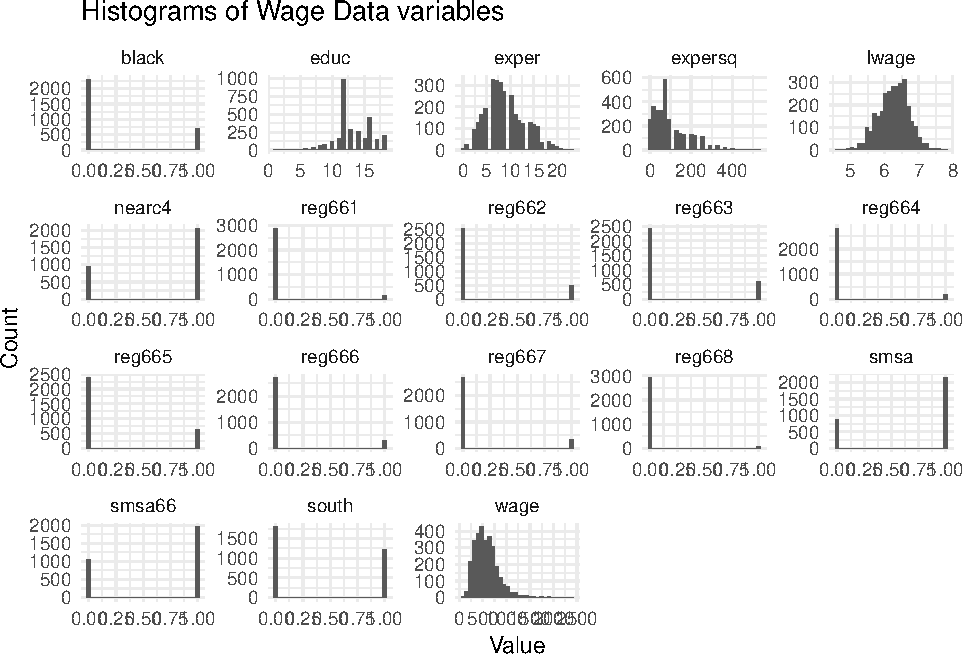
\includegraphics{ps5_code_files/figure-latex/plot_series-1.pdf}

\subsubsection{(b) OLS on log(wage)}\label{b-ols-on-logwage}

\begin{Shaded}
\begin{Highlighting}[]
\NormalTok{rhs_vars <-}\StringTok{ }\KeywordTok{c}\NormalTok{(}\StringTok{"educ"}\NormalTok{, }\StringTok{"exper"}\NormalTok{, }\StringTok{"expersq"}\NormalTok{, }\StringTok{"black"}\NormalTok{, }\StringTok{"south"}\NormalTok{, }\StringTok{"smsa"}\NormalTok{, }\StringTok{"reg661"}\NormalTok{, }\StringTok{"reg662"}\NormalTok{, }\StringTok{"reg663"}\NormalTok{, }\StringTok{"reg664"}\NormalTok{, }\StringTok{"reg665"}\NormalTok{, }\StringTok{"reg666"}\NormalTok{, }\StringTok{"reg667"}\NormalTok{, }\StringTok{"reg668"}\NormalTok{, }\StringTok{"smsa66"}\NormalTok{)}

\NormalTok{model1 <-}\StringTok{ }\KeywordTok{ols}\NormalTok{(card_df, }\StringTok{"lwage"}\NormalTok{, rhs_vars)}

\NormalTok{model1}\OperatorTok{$}\NormalTok{ttest}
\end{Highlighting}
\end{Shaded}

\begin{longtable}[]{@{}lrrrrl@{}}
\caption{OLS Results}\tabularnewline
\toprule
& Coef. & S.E. & t Stat & p-Value & Decision\tabularnewline
\midrule
\endfirsthead
\toprule
& Coef. & S.E. & t Stat & p-Value & Decision\tabularnewline
\midrule
\endhead
intercept & 4.739 & 0.0715 & 66.259 & 0.0000 & Reject\tabularnewline
educ & 0.075 & 0.0035 & 21.351 & 0.0000 & Reject\tabularnewline
exper & 0.085 & 0.0066 & 12.806 & 0.0000 & Reject\tabularnewline
expersq & -0.002 & 0.0003 & -7.223 & 0.0000 & Reject\tabularnewline
black & -0.199 & 0.0182 & -10.906 & 0.0000 & Reject\tabularnewline
south & -0.148 & 0.0260 & -5.695 & 0.0000 & Reject\tabularnewline
smsa & 0.136 & 0.0201 & 6.785 & 0.0000 & Reject\tabularnewline
reg661 & -0.119 & 0.0388 & -3.054 & 0.0023 & Reject\tabularnewline
reg662 & -0.022 & 0.0283 & -0.786 & 0.4321 & Fail to
Reject\tabularnewline
reg663 & 0.026 & 0.0274 & 0.949 & 0.3427 & Fail to Reject\tabularnewline
reg664 & -0.063 & 0.0357 & -1.780 & 0.0753 & Fail to
Reject\tabularnewline
reg665 & 0.009 & 0.0361 & 0.262 & 0.7935 & Fail to Reject\tabularnewline
reg666 & 0.022 & 0.0401 & 0.547 & 0.5842 & Fail to Reject\tabularnewline
reg667 & -0.001 & 0.0394 & -0.015 & 0.9881 & Fail to
Reject\tabularnewline
reg668 & -0.175 & 0.0463 & -3.777 & 0.0002 & Reject\tabularnewline
smsa66 & 0.026 & 0.0194 & 1.349 & 0.1773 & Fail to Reject\tabularnewline
These point & estimates & are very & close to & those of t & he paper.
However, we do not know how to interprent yes/no from the region
(reg661-668) and live in SMSA in 1966 (smsa66) variable in comparison to
our estimate values.\tabularnewline
\bottomrule
\end{longtable}

\subsubsection{(c) Reduced Form}\label{c-reduced-form}

Estimate reduced form equation for \emph{educ} containing all of the
explanatory variables and the dummy variable \emph{nearc4}

\begin{Shaded}
\begin{Highlighting}[]
\NormalTok{rhs_vars <-}\StringTok{ }\KeywordTok{c}\NormalTok{(}\StringTok{"nearc4"}\NormalTok{, }\StringTok{"exper"}\NormalTok{, }\StringTok{"expersq"}\NormalTok{, }\StringTok{"black"}\NormalTok{, }\StringTok{"south"}\NormalTok{, }\StringTok{"smsa"}\NormalTok{, }\StringTok{"reg661"}\NormalTok{, }\StringTok{"reg662"}\NormalTok{, }\StringTok{"reg663"}\NormalTok{, }\StringTok{"reg664"}\NormalTok{, }\StringTok{"reg665"}\NormalTok{, }\StringTok{"reg666"}\NormalTok{, }\StringTok{"reg667"}\NormalTok{, }\StringTok{"reg668"}\NormalTok{, }\StringTok{"smsa66"}\NormalTok{)}

\NormalTok{rf <-}\StringTok{ }\KeywordTok{ols}\NormalTok{(card_df, }\StringTok{"educ"}\NormalTok{, rhs_vars)}

\NormalTok{rf}\OperatorTok{$}\NormalTok{ttest}
\end{Highlighting}
\end{Shaded}

\begin{longtable}[]{@{}lrrrrl@{}}
\caption{OLS Results}\tabularnewline
\toprule
& Coef. & S.E. & t Stat & p-Value & Decision\tabularnewline
\midrule
\endfirsthead
\toprule
& Coef. & S.E. & t Stat & p-Value & Decision\tabularnewline
\midrule
\endhead
intercept & 16.849 & 0.2111 & 79.805 & 0.0000 & Reject\tabularnewline
nearc4 & 0.320 & 0.0879 & 3.641 & 0.0003 & Reject\tabularnewline
exper & -0.413 & 0.0337 & -12.241 & 0.0000 & Reject\tabularnewline
expersq & 0.001 & 0.0017 & 0.526 & 0.5987 & Fail to
Reject\tabularnewline
black & -0.936 & 0.0937 & -9.981 & 0.0000 & Reject\tabularnewline
south & -0.052 & 0.1354 & -0.381 & 0.7032 & Fail to
Reject\tabularnewline
smsa & 0.402 & 0.1048 & 3.837 & 0.0001 & Reject\tabularnewline
reg661 & -0.210 & 0.2025 & -1.039 & 0.2991 & Fail to
Reject\tabularnewline
reg662 & -0.289 & 0.1473 & -1.961 & 0.0500 & Reject\tabularnewline
reg663 & -0.238 & 0.1426 & -1.670 & 0.0950 & Fail to
Reject\tabularnewline
reg664 & -0.093 & 0.1860 & -0.501 & 0.6167 & Fail to
Reject\tabularnewline
reg665 & -0.483 & 0.1882 & -2.566 & 0.0103 & Reject\tabularnewline
reg666 & -0.513 & 0.2096 & -2.448 & 0.0144 & Reject\tabularnewline
reg667 & -0.427 & 0.2056 & -2.077 & 0.0379 & Reject\tabularnewline
reg668 & 0.314 & 0.2417 & 1.298 & 0.1945 & Fail to Reject\tabularnewline
smsa66 & 0.025 & 0.1058 & 0.241 & 0.8096 & Fail to Reject\tabularnewline
\bottomrule
\end{longtable}

Yes, the partial correlation between \emph{educ} and \emph{nearc4} IS
statistically significant!

\subsubsection{(d) Single IV}\label{d-single-iv}

Estimate the \emph{log(wage)} equation by instrumental variables, using
\emph{nearc4} as an instrument for \emph{educ}.

Compare the 95\% confidence interval for the return to educutioan to
that obtained from the Least Squares regression above.

\begin{Shaded}
\begin{Highlighting}[]
\NormalTok{iv <-}\StringTok{ }\ControlFlowTok{function}\NormalTok{(data, y_var, X_vars, Z_vars, }\DataTypeTok{intercept =}\NormalTok{ T, }\DataTypeTok{hetsked =}\NormalTok{ T, }\DataTypeTok{alpha =} \FloatTok{0.05}\NormalTok{) \{}
\NormalTok{    y <-}\StringTok{ }\KeywordTok{to_matrix}\NormalTok{ (}\DataTypeTok{the_df =}\NormalTok{ data, }\DataTypeTok{vars =}\NormalTok{ y_vars)}
\NormalTok{    X <-}\StringTok{ }\KeywordTok{to_matrix}\NormalTok{ (}\DataTypeTok{the_df =}\NormalTok{ data, }\DataTypeTok{vars =}\NormalTok{ X_vars)}
\NormalTok{    Z <-}\StringTok{ }\KeywordTok{to_matrix}\NormalTok{ (}\DataTypeTok{the_df =}\NormalTok{ data, }\DataTypeTok{vars =}\NormalTok{ Z_vars)}
  
  \CommentTok{# Add intercept}
  \ControlFlowTok{if}\NormalTok{ (intercept }\OperatorTok{==}\StringTok{ }\NormalTok{T) X <-}\StringTok{ }\KeywordTok{cbind}\NormalTok{(}\DecValTok{1}\NormalTok{, X)}
  \ControlFlowTok{if}\NormalTok{ (intercept }\OperatorTok{==}\StringTok{ }\NormalTok{T) Z <-}\StringTok{ }\KeywordTok{cbind}\NormalTok{(}\DecValTok{1}\NormalTok{, Z)}
  \CommentTok{# Calculate n and k for degrees of freedom}
\NormalTok{  n <-}\StringTok{ }\KeywordTok{nrow}\NormalTok{(X)}
\NormalTok{  k <-}\StringTok{ }\KeywordTok{ncol}\NormalTok{(X)}
  \CommentTok{# Estimate coefficients}
\NormalTok{  b <-}\StringTok{ }\KeywordTok{solve}\NormalTok{(}\KeywordTok{t}\NormalTok{(Z) }\OperatorTok\StringTok{ }\NormalTok{X) }\OperatorTok\StringTok{ }\KeywordTok{t}\NormalTok{(Z) }\OperatorTok\StringTok{ }\NormalTok{y}
  \CommentTok{# Update names}
  \ControlFlowTok{if}\NormalTok{ (intercept }\OperatorTok{==}\StringTok{ }\NormalTok{T) }\KeywordTok{rownames}\NormalTok{(b)[}\DecValTok{1}\NormalTok{] <-}\StringTok{ "Intercept"} \CommentTok{# Calculate OLS residuals}
\NormalTok{  e <-}\StringTok{ }\NormalTok{y }\OperatorTok{-}\StringTok{ }\NormalTok{X }\OperatorTok\StringTok{ }\NormalTok{b}
\NormalTok{  s2 <-}\StringTok{ }\NormalTok{(}\KeywordTok{t}\NormalTok{(e) }\OperatorTok\StringTok{ }\NormalTok{e) }\OperatorTok{/}\StringTok{ }\NormalTok{(n}\OperatorTok{-}\NormalTok{k)}
  
  \CommentTok{# Calculate X_hat}
\NormalTok{  X_hat <-}\StringTok{ }\NormalTok{Z }\OperatorTok\StringTok{ }\KeywordTok{solve}\NormalTok{(}\KeywordTok{t}\NormalTok{(Z) }\OperatorTok\StringTok{ }\NormalTok{Z) }\OperatorTok\StringTok{ }\KeywordTok{t}\NormalTok{(Z) }\OperatorTok\StringTok{ }\NormalTok{X }
  \CommentTok{# Calculate the inverse of X_hat'X_hat}
\NormalTok{  XX <-}\StringTok{ }\KeywordTok{t}\NormalTok{(X_hat) }\OperatorTok\StringTok{ }\NormalTok{X_hat}
  \CommentTok{# Inverse of X'X}
\NormalTok{  XX_inv <-}\StringTok{ }\KeywordTok{solve}\NormalTok{(XX)}
  \CommentTok{# Calculate the variance-covariance matrix}
  \ControlFlowTok{if}\NormalTok{ (hetsked }\OperatorTok{==}\StringTok{ }\NormalTok{T) \{}
\NormalTok{    sigma_hat <-}\StringTok{ }\KeywordTok{lapply}\NormalTok{(}\DataTypeTok{X =} \DecValTok{1}\OperatorTok{:}\NormalTok{n, }\DataTypeTok{FUN =} \ControlFlowTok{function}\NormalTok{(i) \{}
      \CommentTok{# Define x_i}
\NormalTok{      x_i <-}\StringTok{ }\KeywordTok{matrix}\NormalTok{(}\KeywordTok{as.vector}\NormalTok{(X_hat[i,]), }\DataTypeTok{nrow =} \DecValTok{1}\NormalTok{) }\CommentTok{# Return x_i' x_i e_i^2}
      \KeywordTok{return}\NormalTok{(}\KeywordTok{t}\NormalTok{(x_i) }\OperatorTok\StringTok{ }\NormalTok{x_i }\OperatorTok{*}\StringTok{ }\NormalTok{e[i]}\OperatorTok{^}\DecValTok{2}\NormalTok{)}
\NormalTok{    \}) }\OperatorTok\StringTok{ }\KeywordTok{Reduce}\NormalTok{(}\DataTypeTok{f =} \StringTok{"+"}\NormalTok{, }\DataTypeTok{x =}\NormalTok{ .) }
\NormalTok{  \}}
  
  \ControlFlowTok{if}\NormalTok{ (hetsked }\OperatorTok{==}\StringTok{ }\NormalTok{F) sigma_hat <-}\StringTok{ }\NormalTok{XX}
  \CommentTok{# Calculate the standard error}
\NormalTok{  se <-}\StringTok{ }\KeywordTok{sqrt}\NormalTok{(s2 }\OperatorTok{*}\StringTok{ }\KeywordTok{diag}\NormalTok{(XX_inv }\OperatorTok\StringTok{ }\NormalTok{sigma_hat }\OperatorTok\StringTok{ }\NormalTok{XX_inv)) }\CommentTok{# Vector of _t_ statistics}
\NormalTok{  t_stats <-}\StringTok{ }\NormalTok{(b }\OperatorTok{-}\StringTok{ }\DecValTok{0}\NormalTok{) }\OperatorTok{/}\StringTok{ }\NormalTok{se}
  \CommentTok{# Calculate the p-values}
\NormalTok{  p_values =}\StringTok{ }\KeywordTok{pt}\NormalTok{(}\DataTypeTok{q =} \KeywordTok{abs}\NormalTok{(t_stats), }\DataTypeTok{df =}\NormalTok{ n}\OperatorTok{-}\NormalTok{k, }\DataTypeTok{lower.tail =}\NormalTok{ F) }\OperatorTok{*}\StringTok{ }\DecValTok{2} \CommentTok{# Names for coefficients}
\NormalTok{  var_names <-}\StringTok{ }\NormalTok{X_vars}
  \ControlFlowTok{if}\NormalTok{ (intercept }\OperatorTok{==}\StringTok{ }\NormalTok{T) var_names <-}\StringTok{ }\KeywordTok{c}\NormalTok{(}\StringTok{"Intercept"}\NormalTok{, var_names)}
  
    \CommentTok{# t-test----}
    \CommentTok{# Do we (fail to) reject?}
\NormalTok{    reject <-}\StringTok{ }\KeywordTok{ifelse}\NormalTok{(p_values }\OperatorTok{<}\StringTok{ }\NormalTok{alpha, reject <-}\StringTok{ "Reject"}\NormalTok{, reject <-}\StringTok{ "Fail to Reject"}\NormalTok{)}
    \CommentTok{# Nice table (data.frame) of results}
\NormalTok{    results <-}\StringTok{ }\KeywordTok{data.frame}\NormalTok{(}
      \CommentTok{# The rows have the coef. names}
      \DataTypeTok{effect =} \KeywordTok{rownames}\NormalTok{(b),}
      \CommentTok{# Estimated coefficients}
      \DataTypeTok{coef =} \KeywordTok{as.vector}\NormalTok{(b) }\OperatorTok\StringTok{ }\KeywordTok{round}\NormalTok{(}\DecValTok{3}\NormalTok{),}
      \CommentTok{# Standard errors}
      \DataTypeTok{std_error =} \KeywordTok{as.vector}\NormalTok{(se) }\OperatorTok\StringTok{ }\KeywordTok{round}\NormalTok{(}\DecValTok{4}\NormalTok{),}
      \CommentTok{# t statistics}
      \DataTypeTok{t_stat =} \KeywordTok{as.vector}\NormalTok{(t_stats) }\OperatorTok\StringTok{ }\KeywordTok{round}\NormalTok{(}\DecValTok{3}\NormalTok{),}
      \CommentTok{# p-values}
      \DataTypeTok{p_value =} \KeywordTok{as.vector}\NormalTok{(p_values) }\OperatorTok\StringTok{ }\KeywordTok{round}\NormalTok{(}\DecValTok{4}\NormalTok{),}
      \CommentTok{# reject null?}
      \DataTypeTok{significance =} \KeywordTok{as.character}\NormalTok{(reject)}
\NormalTok{      )}
  
\NormalTok{    ttest_table <-}\StringTok{  }\NormalTok{results }\OperatorTok\StringTok{ }\NormalTok{knitr}\OperatorTok{::}\KeywordTok{kable}\NormalTok{(}
      \DataTypeTok{col.names =} \KeywordTok{c}\NormalTok{(}\StringTok{""}\NormalTok{, }\StringTok{"Coef."}\NormalTok{, }\StringTok{"S.E."}\NormalTok{, }\StringTok{"t Stat"}\NormalTok{, }\StringTok{"p-Value"}\NormalTok{, }\StringTok{"Decision"}\NormalTok{),}
      \DataTypeTok{booktabs =}\NormalTok{ T,}
      \DataTypeTok{format.args =} \KeywordTok{list}\NormalTok{(}\DataTypeTok{scientific =}\NormalTok{ F),}
      \DataTypeTok{escape =}\NormalTok{ F,}
      \DataTypeTok{caption =} \StringTok{"IV-OLS Results"}\NormalTok{)}
  
  \KeywordTok{return}\NormalTok{(ttest_table)}
\NormalTok{\}}

\NormalTok{Z_vars <-}\StringTok{ }\KeywordTok{c}\NormalTok{(}\StringTok{"nearc4"}\NormalTok{, }\StringTok{"exper"}\NormalTok{, }\StringTok{"expersq"}\NormalTok{, }\StringTok{"black"}\NormalTok{, }\StringTok{"south"}\NormalTok{, }\StringTok{"smsa"}\NormalTok{, }\StringTok{"reg661"}\NormalTok{, }\StringTok{"reg662"}\NormalTok{, }\StringTok{"reg663"}\NormalTok{, }\StringTok{"reg664"}\NormalTok{, }\StringTok{"reg665"}\NormalTok{, }\StringTok{"reg666"}\NormalTok{, }\StringTok{"reg667"}\NormalTok{, }\StringTok{"reg668"}\NormalTok{, }\StringTok{"smsa66"}\NormalTok{)}
\NormalTok{y_vars <-}\StringTok{ }\KeywordTok{c}\NormalTok{(}\StringTok{"lwage"}\NormalTok{)}
\NormalTok{X_vars <-}\StringTok{ }\KeywordTok{c}\NormalTok{(}\StringTok{"educ"}\NormalTok{, }\StringTok{"exper"}\NormalTok{, }\StringTok{"expersq"}\NormalTok{, }\StringTok{"black"}\NormalTok{, }\StringTok{"south"}\NormalTok{, }\StringTok{"smsa"}\NormalTok{, }\StringTok{"reg661"}\NormalTok{, }\StringTok{"reg662"}\NormalTok{, }\StringTok{"reg663"}\NormalTok{, }\StringTok{"reg664"}\NormalTok{, }\StringTok{"reg665"}\NormalTok{, }\StringTok{"reg666"}\NormalTok{, }\StringTok{"reg667"}\NormalTok{, }\StringTok{"reg668"}\NormalTok{, }\StringTok{"smsa66"}\NormalTok{)}
\CommentTok{# # Run OLS}
\NormalTok{(iv1 <-}\StringTok{ }\KeywordTok{iv}\NormalTok{(card_df, y_vars, X_vars, Z_vars, T, T))}
\end{Highlighting}
\end{Shaded}

\begin{verbatim}
## Warning in s2 * diag(XX_inv %*% sigma_hat %*% XX_inv): Recycling array of length 1 in array-vector arithmetic is deprecated.
##   Use c() or as.vector() instead.
\end{verbatim}

\begin{longtable}[]{@{}lrrrrl@{}}
\caption{IV-OLS Results}\tabularnewline
\toprule
& Coef. & S.E. & t Stat & p-Value & Decision\tabularnewline
\midrule
\endfirsthead
\toprule
& Coef. & S.E. & t Stat & p-Value & Decision\tabularnewline
\midrule
\endhead
Intercept & 3.774 & 0.3563 & 10.593 & 0.0000 & Reject\tabularnewline
educ & 0.132 & 0.0210 & 6.271 & 0.0000 & Reject\tabularnewline
exper & 0.108 & 0.0091 & 11.942 & 0.0000 & Reject\tabularnewline
expersq & -0.002 & 0.0001 & -17.286 & 0.0000 & Reject\tabularnewline
black & -0.147 & 0.0203 & -7.218 & 0.0000 & Reject\tabularnewline
south & -0.145 & 0.0113 & -12.818 & 0.0000 & Reject\tabularnewline
smsa & 0.112 & 0.0121 & 9.269 & 0.0000 & Reject\tabularnewline
reg661 & -0.108 & 0.0159 & -6.777 & 0.0000 & Reject\tabularnewline
reg662 & -0.007 & 0.0131 & -0.538 & 0.5903 & Fail to
Reject\tabularnewline
reg663 & 0.040 & 0.0126 & 3.203 & 0.0014 & Reject\tabularnewline
reg664 & -0.058 & 0.0152 & -3.804 & 0.0001 & Reject\tabularnewline
reg665 & 0.038 & 0.0192 & 2.002 & 0.0454 & Reject\tabularnewline
reg666 & 0.055 & 0.0202 & 2.721 & 0.0065 & Reject\tabularnewline
reg667 & 0.027 & 0.0195 & 1.375 & 0.1692 & Fail to Reject\tabularnewline
reg668 & -0.191 & 0.0197 & -9.698 & 0.0000 & Reject\tabularnewline
smsa66 & 0.019 & 0.0080 & 2.327 & 0.0201 & Reject\tabularnewline
\bottomrule
\end{longtable}

\begin{Shaded}
\begin{Highlighting}[]
\CommentTok{# Compare 95% confidence interval for return on education using nearc4 has IV to that of the OLS above (model_1)}

\NormalTok{iv_b <-}\StringTok{ }\FloatTok{0.1315038}
\NormalTok{iv_se <-}\StringTok{ }\FloatTok{0.0210}

\NormalTok{ols_b <-}\StringTok{ }\FloatTok{0.075}
\NormalTok{ols_se <-}\StringTok{ }\FloatTok{0.0035}

\NormalTok{CI <-}\StringTok{ }\ControlFlowTok{function}\NormalTok{(b, se, }\DataTypeTok{alpha=}\FloatTok{1.96}\NormalTok{) \{}
\NormalTok{  CI <-}\StringTok{ }\KeywordTok{list}\NormalTok{((b }\OperatorTok{-}\StringTok{ }\NormalTok{alpha}\OperatorTok{*}\NormalTok{se), (b }\OperatorTok{+}\StringTok{ }\NormalTok{alpha}\OperatorTok{*}\NormalTok{se))}
  \KeywordTok{return}\NormalTok{(CI)}
\NormalTok{\}}

\KeywordTok{CI}\NormalTok{(iv_b, iv_se) }\OperatorTok\StringTok{ }\NormalTok{knitr}\OperatorTok{::}\KeywordTok{kable}\NormalTok{(}\DataTypeTok{caption =} \StringTok{"Return using nearcr as instrument"}\NormalTok{)}
\end{Highlighting}
\end{Shaded}

\begin{table}
\caption{Return using nearcr as instrument}

\centering
\begin{tabular}[t]{r}
\hline
x\\
\hline
0.0903438\\
\hline
\end{tabular}
\centering
\begin{tabular}[t]{r}
\hline
x\\
\hline
0.1726638\\
\hline
\end{tabular}
\end{table}

\begin{Shaded}
\begin{Highlighting}[]
\KeywordTok{CI}\NormalTok{(ols_b, ols_se) }\OperatorTok\StringTok{ }\NormalTok{knitr}\OperatorTok{::}\KeywordTok{kable}\NormalTok{(}\DataTypeTok{caption =} \StringTok{"Return on education"}\NormalTok{)}
\end{Highlighting}
\end{Shaded}

\begin{table}
\caption{Return on education}

\centering
\begin{tabular}[t]{r}
\hline
x\\
\hline
0.06814\\
\hline
\end{tabular}
\centering
\begin{tabular}[t]{r}
\hline
x\\
\hline
0.08186\\
\hline
\end{tabular}
\end{table}

Wider confidence intervals using \emph{near4c} as IV than in the
original model. The 95\% confidence interval using the instrument is
{[}0.0903, 0.1727{]}, while from OLS it was {[}0.0681,0.0819{]}.

First bring in functions for Whites Heteroskedasticity robust
estimators.

\begin{Shaded}
\begin{Highlighting}[]
\NormalTok{vcov_white <-}\StringTok{ }\ControlFlowTok{function}\NormalTok{(data, y_var, X_vars, }\DataTypeTok{intercept =}\NormalTok{ T) \{}
  \CommentTok{# Turn data into matrices}
\NormalTok{  y <-}\StringTok{ }\KeywordTok{to_matrix}\NormalTok{(data, y_var)}
\NormalTok{  X <-}\StringTok{ }\KeywordTok{to_matrix}\NormalTok{(data, X_vars)}
  \CommentTok{# Add intercept}
  \ControlFlowTok{if}\NormalTok{ (intercept }\OperatorTok{==}\StringTok{ }\NormalTok{T) X <-}\StringTok{ }\KeywordTok{cbind}\NormalTok{(}\DecValTok{1}\NormalTok{, X)}
  \CommentTok{# Calculate n and k for degrees of freedom}
\NormalTok{  n <-}\StringTok{ }\KeywordTok{nrow}\NormalTok{(X)}
\NormalTok{  k <-}\StringTok{ }\KeywordTok{ncol}\NormalTok{(X)}
  \CommentTok{# Estimate coefficients}
\NormalTok{  b <-}\StringTok{ }\KeywordTok{b_ols}\NormalTok{(y, X)}
  \CommentTok{# Update names}
  \ControlFlowTok{if}\NormalTok{ (intercept }\OperatorTok{==}\StringTok{ }\NormalTok{T) }\KeywordTok{rownames}\NormalTok{(b)[}\DecValTok{1}\NormalTok{] <-}\StringTok{ "Intercept"}
  \CommentTok{# Calculate OLS residuals}
\NormalTok{  e <-}\StringTok{ }\NormalTok{y }\OperatorTok{-}\StringTok{ }\NormalTok{X }\OperatorTok\StringTok{ }\NormalTok{b}
  \CommentTok{# Inverse of X'X}
\NormalTok{  XX_inv <-}\StringTok{ }\KeywordTok{solve}\NormalTok{(}\KeywordTok{t}\NormalTok{(X) }\OperatorTok\StringTok{ }\NormalTok{X)}
  \CommentTok{# For each row, calculate x_i' x_i e_i^2; then sum}
\NormalTok{  sigma_hat <-}\StringTok{ }\KeywordTok{lapply}\NormalTok{(}\DataTypeTok{X =} \DecValTok{1}\OperatorTok{:}\NormalTok{n, }\DataTypeTok{FUN =} \ControlFlowTok{function}\NormalTok{(i) \{}
    \CommentTok{# Define x_i}
\NormalTok{    x_i <-}\StringTok{ }\KeywordTok{matrix}\NormalTok{(}\KeywordTok{as.vector}\NormalTok{(X[i,]), }\DataTypeTok{nrow =} \DecValTok{1}\NormalTok{)}
    \CommentTok{# Return x_i' x_i e_i^2}
    \KeywordTok{return}\NormalTok{(}\KeywordTok{t}\NormalTok{(x_i) }\OperatorTok\StringTok{ }\NormalTok{x_i }\OperatorTok{*}\StringTok{ }\NormalTok{e[i]}\OperatorTok{^}\DecValTok{2}\NormalTok{)}
\NormalTok{  \}) }\OperatorTok\StringTok{ }\KeywordTok{Reduce}\NormalTok{(}\DataTypeTok{f =} \StringTok{"+"}\NormalTok{, }\DataTypeTok{x =}\NormalTok{ .)}
  \CommentTok{# Return the results}
  \KeywordTok{return}\NormalTok{(XX_inv }\OperatorTok\StringTok{ }\NormalTok{sigma_hat }\OperatorTok\StringTok{ }\NormalTok{XX_inv)}
\NormalTok{\}}
\end{Highlighting}
\end{Shaded}

\subsubsection{(e) Multiple IV}\label{e-multiple-iv}

Use \emph{nearc2} and \emph{nearc4} as instruments for \emph{educ.}

First, lets build a function for two stage least squares (2SLS or TSLS)
- Multiple Instruments

\begin{Shaded}
\begin{Highlighting}[]
\NormalTok{b_2sls <-}\StringTok{ }\ControlFlowTok{function}\NormalTok{(data, y_var, X_vars, Z_vars, }\DataTypeTok{intercept =}\NormalTok{ T) \{}
  \CommentTok{# Turn data into matrices}
\NormalTok{  y <-}\StringTok{ }\KeywordTok{to_matrix}\NormalTok{(data, y_var)}
\NormalTok{  X <-}\StringTok{ }\KeywordTok{to_matrix}\NormalTok{(data, X_vars)}
\NormalTok{  Z <-}\StringTok{ }\KeywordTok{to_matrix}\NormalTok{(data, Z_vars)}
  \CommentTok{# Add intercept}
  \ControlFlowTok{if}\NormalTok{ (intercept }\OperatorTok{==}\StringTok{ }\NormalTok{T) X <-}\StringTok{ }\KeywordTok{cbind}\NormalTok{(}\DecValTok{1}\NormalTok{, X)}
  \ControlFlowTok{if}\NormalTok{ (intercept }\OperatorTok{==}\StringTok{ }\NormalTok{T) Z <-}\StringTok{ }\KeywordTok{cbind}\NormalTok{(}\DecValTok{1}\NormalTok{, Z)}
  \CommentTok{# Estimate the first stage}
\NormalTok{  b_stage1 <-}\StringTok{ }\KeywordTok{solve}\NormalTok{(}\KeywordTok{t}\NormalTok{(Z) }\OperatorTok\StringTok{ }\NormalTok{Z) }\OperatorTok\StringTok{ }\KeywordTok{t}\NormalTok{(Z) }\OperatorTok\StringTok{ }\NormalTok{X}
  \CommentTok{# Fit the first stage values}
\NormalTok{  X_hat <-}\StringTok{ }\NormalTok{Z }\OperatorTok\StringTok{ }\NormalTok{b_stage1}
  \CommentTok{# Estimate the second stage}
\NormalTok{  b_stage2 <-}\StringTok{ }\KeywordTok{solve}\NormalTok{(}\KeywordTok{t}\NormalTok{(X_hat) }\OperatorTok\StringTok{ }\NormalTok{X_hat) }\OperatorTok\StringTok{ }\KeywordTok{t}\NormalTok{(X_hat) }\OperatorTok\StringTok{ }\NormalTok{y}
  \CommentTok{# Update names}
  \ControlFlowTok{if}\NormalTok{ (intercept }\OperatorTok{==}\StringTok{ }\NormalTok{T) }\KeywordTok{rownames}\NormalTok{(b_stage2)[}\DecValTok{1}\NormalTok{] <-}\StringTok{ "Intercept"}
  \CommentTok{# Return beta_hat}
  \KeywordTok{return}\NormalTok{(b_stage2)}
\NormalTok{\}}
\end{Highlighting}
\end{Shaded}

\begin{Shaded}
\begin{Highlighting}[]
\NormalTok{tsls <-}\StringTok{ }\ControlFlowTok{function}\NormalTok{(data, y_vars, X_vars, Z_vars, }\DataTypeTok{intercept =}\NormalTok{ T, }\DataTypeTok{hetsked =}\NormalTok{ F) \{}
  
  \CommentTok{# Turn data into matrices}
\NormalTok{  y <-}\StringTok{ }\KeywordTok{to_matrix}\NormalTok{(data, y_vars)}
\NormalTok{  X <-}\StringTok{ }\KeywordTok{to_matrix}\NormalTok{(data, X_vars)}
\NormalTok{  Z <-}\StringTok{ }\KeywordTok{to_matrix}\NormalTok{(data, Z_vars)}
  \CommentTok{# Calculate n and k for degrees of freedom}
\NormalTok{  n <-}\StringTok{ }\KeywordTok{nrow}\NormalTok{(X)}
\NormalTok{  k <-}\StringTok{ }\KeywordTok{ncol}\NormalTok{(X)}
  \CommentTok{# Add intercept}
  \ControlFlowTok{if}\NormalTok{ (intercept }\OperatorTok{==}\StringTok{ }\NormalTok{T) X <-}\StringTok{ }\KeywordTok{cbind}\NormalTok{(}\DecValTok{1}\NormalTok{, X)}
  \ControlFlowTok{if}\NormalTok{ (intercept }\OperatorTok{==}\StringTok{ }\NormalTok{T) Z <-}\StringTok{ }\KeywordTok{cbind}\NormalTok{(}\DecValTok{1}\NormalTok{, Z)}
  
\NormalTok{  redform <-}\StringTok{ }\KeywordTok{ols}\NormalTok{(data, y_vars, Z_vars, intercept, hetsked)}\OperatorTok{$}\NormalTok{ttest}
  
  \CommentTok{# First stage}
\NormalTok{  b_stage1 <-}\StringTok{ }\KeywordTok{solve}\NormalTok{(}\KeywordTok{t}\NormalTok{(Z) }\OperatorTok\StringTok{ }\NormalTok{Z) }\OperatorTok\StringTok{ }\KeywordTok{t}\NormalTok{(Z) }\OperatorTok\StringTok{ }\NormalTok{X}
  \CommentTok{# Fit the first stage values}
\NormalTok{  X_hat <-}\StringTok{ }\NormalTok{Z }\OperatorTok\StringTok{ }\NormalTok{b_stage1}
  \CommentTok{# Estimate the second stage}
\NormalTok{  b_stage2 <-}\StringTok{ }\KeywordTok{solve}\NormalTok{(}\KeywordTok{t}\NormalTok{(X_hat) }\OperatorTok\StringTok{ }\NormalTok{X_hat) }\OperatorTok\StringTok{ }\KeywordTok{t}\NormalTok{(X_hat) }\OperatorTok\StringTok{ }\NormalTok{y}
 
   \CommentTok{# INCORRECT STANDARD ERRORS -- use X_hat}
\NormalTok{  e_inc <-}\StringTok{ }\NormalTok{y }\OperatorTok{-}\StringTok{ }\NormalTok{X_hat }\OperatorTok\StringTok{ }\NormalTok{b_stage2}
\NormalTok{  s2_inc <-}\StringTok{ }\NormalTok{(}\KeywordTok{t}\NormalTok{(e_inc) }\OperatorTok\StringTok{ }\NormalTok{e_inc) }\OperatorTok{/}\StringTok{ }\NormalTok{(n}\OperatorTok{-}\NormalTok{k)}
\NormalTok{  s2_inc }\OperatorTok\StringTok{ }\KeywordTok{as.numeric}\NormalTok{()}
\NormalTok{  XX_inv <-}\StringTok{ }\KeywordTok{solve}\NormalTok{(}\KeywordTok{t}\NormalTok{(X_hat) }\OperatorTok\StringTok{ }\NormalTok{X_hat)}
\NormalTok{  se_inc <-}\StringTok{ }\KeywordTok{sqrt}\NormalTok{(s2_inc }\OperatorTok{*}\StringTok{ }\KeywordTok{diag}\NormalTok{(XX_inv))}
  
  \CommentTok{# Update names}
  \ControlFlowTok{if}\NormalTok{ (intercept }\OperatorTok{==}\StringTok{ }\NormalTok{T) }\KeywordTok{rownames}\NormalTok{(b_stage2)[}\DecValTok{1}\NormalTok{] <-}\StringTok{ "Intercept"}
  
  
  \CommentTok{# Calculate P_Z}
\NormalTok{  P_Z <-}\StringTok{ }\NormalTok{Z }\OperatorTok\StringTok{ }\KeywordTok{solve}\NormalTok{(}\KeywordTok{t}\NormalTok{(Z) }\OperatorTok\StringTok{ }\NormalTok{Z) }\OperatorTok\StringTok{ }\KeywordTok{t}\NormalTok{(Z)}
  \CommentTok{# Calculate b_2sls}
\NormalTok{  b <-}\StringTok{ }\KeywordTok{solve}\NormalTok{(}\KeywordTok{t}\NormalTok{(X) }\OperatorTok\StringTok{ }\NormalTok{P_Z }\OperatorTok\StringTok{ }\NormalTok{X) }\OperatorTok\StringTok{ }\KeywordTok{t}\NormalTok{(X) }\OperatorTok\StringTok{ }\NormalTok{P_Z }\OperatorTok\StringTok{ }\NormalTok{y}
  \CommentTok{# Calculate OLS residuals}
\NormalTok{  e <-}\StringTok{ }\NormalTok{y }\OperatorTok{-}\StringTok{ }\NormalTok{X }\OperatorTok\StringTok{ }\NormalTok{b}
  \CommentTok{# Calculate s^2}
\NormalTok{  s2 <-}\StringTok{ }\NormalTok{(}\KeywordTok{t}\NormalTok{(e) }\OperatorTok\StringTok{ }\NormalTok{e) }\OperatorTok{/}\StringTok{ }\NormalTok{(n }\OperatorTok{-}\StringTok{ }\NormalTok{k)   }
\NormalTok{  s2 }\OperatorTok\StringTok{ }\KeywordTok{as.numeric}\NormalTok{()}
  \CommentTok{# Inverse of X' Pz X}
\NormalTok{  XX_inv <-}\StringTok{ }\KeywordTok{solve}\NormalTok{(}\KeywordTok{t}\NormalTok{(X) }\OperatorTok\StringTok{ }\NormalTok{P_Z }\OperatorTok\StringTok{ }\NormalTok{X)}
  \CommentTok{# Standard error}
\NormalTok{  se <-}\StringTok{ }\KeywordTok{sqrt}\NormalTok{(s2 }\OperatorTok{*}\StringTok{ }\KeywordTok{diag}\NormalTok{(XX_inv))    }\CommentTok{# These should be the 'correct' standard errors}
  \CommentTok{# Vector of _t_ statistics}
\NormalTok{  t_stats <-}\StringTok{ }\NormalTok{(b }\OperatorTok{-}\StringTok{ }\DecValTok{0}\NormalTok{) }\OperatorTok{/}\StringTok{ }\NormalTok{se}
\NormalTok{  t_stats_inc <-}\StringTok{ }\NormalTok{(b }\OperatorTok{-}\StringTok{ }\DecValTok{0}\NormalTok{) }\OperatorTok{/}\StringTok{ }\NormalTok{se_inc}
  \CommentTok{# Calculate the p-values}
\NormalTok{  p_values =}\StringTok{ }\KeywordTok{pt}\NormalTok{(}\DataTypeTok{q =} \KeywordTok{abs}\NormalTok{(t_stats), }\DataTypeTok{df =}\NormalTok{ n}\OperatorTok{-}\NormalTok{k, }\DataTypeTok{lower.tail =}\NormalTok{ F) }\OperatorTok{*}\StringTok{ }\DecValTok{2}
\NormalTok{  p_values_inc =}\StringTok{ }\KeywordTok{pt}\NormalTok{(}\DataTypeTok{q =} \KeywordTok{abs}\NormalTok{(t_stats_inc), }\DataTypeTok{df =}\NormalTok{ n}\OperatorTok{-}\NormalTok{k, }\DataTypeTok{lower.tail =}\NormalTok{ F) }\OperatorTok{*}\StringTok{ }\DecValTok{2}

  \CommentTok{# Update names}
  \ControlFlowTok{if}\NormalTok{ (intercept }\OperatorTok{==}\StringTok{ }\NormalTok{T) }\KeywordTok{rownames}\NormalTok{(b)[}\DecValTok{1}\NormalTok{] <-}\StringTok{ "Intercept"}
  
  \CommentTok{# Nice table (data.frame) of CORRECT results}
\NormalTok{  correct_res <-}\StringTok{ }\KeywordTok{data.frame}\NormalTok{(}
    \CommentTok{# The rows have the coef. names}
    \DataTypeTok{effect =} \KeywordTok{rownames}\NormalTok{(b),}
    \CommentTok{# Estimated coefficients}
    \DataTypeTok{coef =} \KeywordTok{as.vector}\NormalTok{(b),}
    \CommentTok{# Standard errors}
    \DataTypeTok{std_error =} \KeywordTok{as.vector}\NormalTok{(se),}
    \CommentTok{# t statistics}
    \DataTypeTok{t_stat =} \KeywordTok{as.vector}\NormalTok{(t_stats),}
    \CommentTok{# p-values}
    \DataTypeTok{p_value =} \KeywordTok{as.vector}\NormalTok{(p_values)}
\NormalTok{    )}
  \CommentTok{# INCORRECT RESULTS}
\NormalTok{    incorrect_res <-}\StringTok{ }\KeywordTok{data.frame}\NormalTok{(}
    \DataTypeTok{effect =} \KeywordTok{rownames}\NormalTok{(b),}
    \DataTypeTok{coef =} \KeywordTok{as.vector}\NormalTok{(b),}
    \DataTypeTok{std_error =} \KeywordTok{as.vector}\NormalTok{(se_inc),}
    \CommentTok{# t statistics}
    \DataTypeTok{t_stat =} \KeywordTok{as.vector}\NormalTok{(t_stats_inc),}
    \CommentTok{# p-values}
    \DataTypeTok{p_value =} \KeywordTok{as.vector}\NormalTok{(p_values_inc)}
\NormalTok{  )}

\NormalTok{  results_list <-}\StringTok{ }\KeywordTok{list}\NormalTok{()}
  
  \CommentTok{# Return the results}
  \KeywordTok{return}\NormalTok{(}\KeywordTok{list}\NormalTok{(}\DataTypeTok{correctSE =}\NormalTok{ correct_res, }\DataTypeTok{incorrectSE =}\NormalTok{ incorrect_res, }\DataTypeTok{redform =}\NormalTok{ redform))}
  
\NormalTok{\}}

\NormalTok{Z_vars <-}\StringTok{ }\KeywordTok{c}\NormalTok{(}\StringTok{"nearc4"}\NormalTok{, }\StringTok{"nearc2"}\NormalTok{, }\StringTok{"exper"}\NormalTok{, }\StringTok{"expersq"}\NormalTok{, }\StringTok{"black"}\NormalTok{, }\StringTok{"south"}\NormalTok{, }\StringTok{"smsa"}\NormalTok{, }\StringTok{"reg661"}\NormalTok{, }\StringTok{"reg662"}\NormalTok{, }\StringTok{"reg663"}\NormalTok{, }\StringTok{"reg664"}\NormalTok{, }\StringTok{"reg665"}\NormalTok{, }\StringTok{"reg666"}\NormalTok{, }\StringTok{"reg667"}\NormalTok{, }\StringTok{"reg668"}\NormalTok{, }\StringTok{"smsa66"}\NormalTok{)}
\NormalTok{y_vars <-}\StringTok{ }\KeywordTok{c}\NormalTok{(}\StringTok{"lwage"}\NormalTok{)}
\NormalTok{X_vars <-}\StringTok{ }\KeywordTok{c}\NormalTok{(}\StringTok{"educ"}\NormalTok{, }\StringTok{"exper"}\NormalTok{, }\StringTok{"expersq"}\NormalTok{, }\StringTok{"black"}\NormalTok{, }\StringTok{"south"}\NormalTok{, }\StringTok{"smsa"}\NormalTok{, }\StringTok{"reg661"}\NormalTok{, }\StringTok{"reg662"}\NormalTok{, }\StringTok{"reg663"}\NormalTok{, }\StringTok{"reg664"}\NormalTok{, }\StringTok{"reg665"}\NormalTok{, }\StringTok{"reg666"}\NormalTok{, }\StringTok{"reg667"}\NormalTok{, }\StringTok{"reg668"}\NormalTok{, }\StringTok{"smsa66"}\NormalTok{)}
\end{Highlighting}
\end{Shaded}

\begin{Shaded}
\begin{Highlighting}[]
\CommentTok{#RUN FUNCTION}
\NormalTok{two_stage <-}\StringTok{ }\KeywordTok{tsls}\NormalTok{(}\DataTypeTok{data =}\NormalTok{ card_df, y_vars, X_vars, Z_vars, T, F)}

\CommentTok{# Reduced Form}
\NormalTok{two_stage}\OperatorTok{$}\NormalTok{redform }
\end{Highlighting}
\end{Shaded}

\begin{longtable}[]{@{}lrrrrl@{}}
\caption{OLS Results}\tabularnewline
\toprule
& Coef. & S.E. & t Stat & p-Value & Decision\tabularnewline
\midrule
\endfirsthead
\toprule
& Coef. & S.E. & t Stat & p-Value & Decision\tabularnewline
\midrule
\endhead
intercept & 5.968 & 0.0445 & 134.123 & 0.0000 & Reject\tabularnewline
nearc4 & 0.042 & 0.0181 & 2.340 & 0.0194 & Reject\tabularnewline
nearc2 & 0.036 & 0.0159 & 2.251 & 0.0245 & Reject\tabularnewline
exper & 0.054 & 0.0069 & 7.807 & 0.0000 & Reject\tabularnewline
expersq & -0.002 & 0.0003 & -6.562 & 0.0000 & Reject\tabularnewline
black & -0.273 & 0.0193 & -14.116 & 0.0000 & Reject\tabularnewline
south & -0.149 & 0.0279 & -5.332 & 0.0000 & Reject\tabularnewline
smsa & 0.164 & 0.0216 & 7.632 & 0.0000 & Reject\tabularnewline
reg661 & -0.123 & 0.0420 & -2.940 & 0.0033 & Reject\tabularnewline
reg662 & -0.039 & 0.0304 & -1.291 & 0.1968 & Fail to
Reject\tabularnewline
reg663 & 0.023 & 0.0300 & 0.771 & 0.4409 & Fail to Reject\tabularnewline
reg664 & -0.054 & 0.0389 & -1.389 & 0.1651 & Fail to
Reject\tabularnewline
reg665 & -0.012 & 0.0391 & -0.299 & 0.7648 & Fail to
Reject\tabularnewline
reg666 & -0.009 & 0.0431 & -0.214 & 0.8307 & Fail to
Reject\tabularnewline
reg667 & -0.015 & 0.0428 & -0.350 & 0.7264 & Fail to
Reject\tabularnewline
reg668 & -0.130 & 0.0505 & -2.570 & 0.0102 & Reject\tabularnewline
smsa66 & 0.014 & 0.0220 & 0.658 & 0.5103 & Fail to Reject\tabularnewline
\bottomrule
\end{longtable}

\emph{Comment on the significance of the partial correlations of both
instruments in the reduced form.}

Both instruments (\emph{nearc4} and \emph{nearc2}) show positive and
significant effects.

\emph{Show your standard errors from the second stage and compare them
to the correct standard errors.}

\begin{Shaded}
\begin{Highlighting}[]
\NormalTok{two_stage}\OperatorTok{$}\NormalTok{correctSE }\OperatorTok\StringTok{ }\NormalTok{knitr}\OperatorTok{::}\KeywordTok{kable}\NormalTok{(}\DataTypeTok{caption =} \StringTok{"Correct Standard Errors"}\NormalTok{)}
\end{Highlighting}
\end{Shaded}

\begin{longtable}[]{@{}lrrrr@{}}
\caption{Correct Standard Errors}\tabularnewline
\toprule
effect & coef & std\_error & t\_stat & p\_value\tabularnewline
\midrule
\endfirsthead
\toprule
effect & coef & std\_error & t\_stat & p\_value\tabularnewline
\midrule
\endhead
Intercept & 3.3396875 & 0.8943883 & 3.7340464 & 0.0001919\tabularnewline
educ & 0.1570593 & 0.0525695 & 2.9876535 & 0.0028341\tabularnewline
exper & 0.1188149 & 0.0228023 & 5.2106618 & 0.0000002\tabularnewline
expersq & -0.0023565 & 0.0003475 & -6.7820393 & 0.0000000\tabularnewline
black & -0.1232778 & 0.0521413 & -2.3643020 & 0.0181275\tabularnewline
south & -0.1431945 & 0.0284400 & -5.0349610 & 0.0000005\tabularnewline
smsa & 0.1007530 & 0.0315141 & 3.1970804 & 0.0014027\tabularnewline
reg661 & -0.1029760 & 0.0434151 & -2.3718928 & 0.0177601\tabularnewline
reg662 & -0.0002287 & 0.0337886 & -0.0067676 & 0.9946007\tabularnewline
reg663 & 0.0469556 & 0.0326436 & 1.4384337 & 0.1504155\tabularnewline
reg664 & -0.0554084 & 0.0391763 & -1.4143342 & 0.1573677\tabularnewline
reg665 & 0.0515041 & 0.0475598 & 1.0829330 & 0.2789253\tabularnewline
reg666 & 0.0699968 & 0.0532960 & 1.3133585 & 0.1891628\tabularnewline
reg667 & 0.0390596 & 0.0497416 & 0.7852502 & 0.4323690\tabularnewline
reg668 & -0.1980371 & 0.0525262 & -3.7702521 & 0.0001662\tabularnewline
smsa66 & 0.0150626 & 0.0223322 & 0.6744764 & 0.5000606\tabularnewline
\bottomrule
\end{longtable}

\begin{Shaded}
\begin{Highlighting}[]
\NormalTok{two_stage}\OperatorTok{$}\NormalTok{incorrectSE }\OperatorTok\StringTok{ }\NormalTok{knitr}\OperatorTok{::}\KeywordTok{kable}\NormalTok{(}\DataTypeTok{caption =} \StringTok{"Incorrect Standard Errors"}\NormalTok{)}
\end{Highlighting}
\end{Shaded}

\begin{longtable}[]{@{}lrrrr@{}}
\caption{Incorrect Standard Errors}\tabularnewline
\toprule
effect & coef & std\_error & t\_stat & p\_value\tabularnewline
\midrule
\endfirsthead
\toprule
effect & coef & std\_error & t\_stat & p\_value\tabularnewline
\midrule
\endhead
Intercept & 3.3396875 & 0.8805385 & 3.7927785 & 0.0001519\tabularnewline
educ & 0.1570593 & 0.0517554 & 3.0346457 & 0.0024289\tabularnewline
exper & 0.1188149 & 0.0224492 & 5.2926194 & 0.0000001\tabularnewline
expersq & -0.0023565 & 0.0003421 & -6.8887127 & 0.0000000\tabularnewline
black & -0.1232778 & 0.0513339 & -2.4014897 & 0.0163890\tabularnewline
south & -0.1431945 & 0.0279996 & -5.1141550 & 0.0000003\tabularnewline
smsa & 0.1007530 & 0.0310261 & 3.2473667 & 0.0011776\tabularnewline
reg661 & -0.1029760 & 0.0427428 & -2.4091999 & 0.0160475\tabularnewline
reg662 & -0.0002287 & 0.0332654 & -0.0068741 & 0.9945158\tabularnewline
reg663 & 0.0469556 & 0.0321381 & 1.4610586 & 0.1441043\tabularnewline
reg664 & -0.0554084 & 0.0385696 & -1.4365800 & 0.1509418\tabularnewline
reg665 & 0.0515041 & 0.0468234 & 1.0999663 & 0.2714352\tabularnewline
reg666 & 0.0699968 & 0.0524707 & 1.3340160 & 0.1823000\tabularnewline
reg667 & 0.0390596 & 0.0489713 & 0.7976012 & 0.4251652\tabularnewline
reg668 & -0.1980371 & 0.0517128 & -3.8295537 & 0.0001310\tabularnewline
smsa66 & 0.0150626 & 0.0219864 & 0.6850851 & 0.4933432\tabularnewline
\bottomrule
\end{longtable}

\subsubsection{(f) Hausman test}\label{f-hausman-test}

\emph{Should we worry about endogenaity?} Conduct a Hausman test for
endogeneity of educ. Report your test statistic, critical value and
p-value.

Procedure: 1. Regress endogenous var X on instrument(s) Z. save
residuals as v\_hat 2. Include v\_hat in original model 3. test if
paramater coefficient on v-hat = 0 (ttest)

*Note: This test is only valid asymptotically (and, of course, is only
as good as the instruments used).

\begin{Shaded}
\begin{Highlighting}[]
\NormalTok{Z_vars <-}\StringTok{ }\KeywordTok{c}\NormalTok{(}\StringTok{"exper"}\NormalTok{, }\StringTok{"expersq"}\NormalTok{, }\StringTok{"black"}\NormalTok{, }\StringTok{"south"}\NormalTok{, }\StringTok{"smsa"}\NormalTok{,}
              \StringTok{"smsa66"}\NormalTok{, }\StringTok{"reg661"}\NormalTok{, }\StringTok{"reg662"}\NormalTok{, }\StringTok{"reg663"}\NormalTok{, }\StringTok{"reg664"}\NormalTok{,}
              \StringTok{"reg665"}\NormalTok{, }\StringTok{"reg666"}\NormalTok{, }\StringTok{"reg667"}\NormalTok{, }\StringTok{"reg668"}\NormalTok{, }\StringTok{"nearc4"}\NormalTok{, }\StringTok{"nearc2"}\NormalTok{)}

\NormalTok{card_df }\OperatorTok\StringTok{ }\KeywordTok{mutate}\NormalTok{(}\DataTypeTok{v_hat =} \KeywordTok{ols}\NormalTok{(card_df,}\StringTok{"educ"}\NormalTok{,Z_vars,T,F)}\OperatorTok{$}\NormalTok{vars}\OperatorTok{$}\NormalTok{e)}

\NormalTok{X_vars <-}\StringTok{ }\KeywordTok{c}\NormalTok{(}\StringTok{"educ"}\NormalTok{, }\StringTok{"exper"}\NormalTok{, }\StringTok{"expersq"}\NormalTok{, }\StringTok{"black"}\NormalTok{, }\StringTok{"south"}\NormalTok{, }\StringTok{"smsa"}\NormalTok{, }\StringTok{"reg661"}\NormalTok{, }\StringTok{"reg662"}\NormalTok{, }\StringTok{"reg663"}\NormalTok{, }\StringTok{"reg664"}\NormalTok{, }\StringTok{"reg665"}\NormalTok{, }\StringTok{"reg666"}\NormalTok{, }\StringTok{"reg667"}\NormalTok{, }\StringTok{"reg668"}\NormalTok{, }\StringTok{"smsa66"}\NormalTok{, }\StringTok{"v_hat"}\NormalTok{)}

\NormalTok{orig <-}\StringTok{ }\KeywordTok{ols}\NormalTok{(card_df,}\StringTok{"lwage"}\NormalTok{,X_vars,T,F,}\DataTypeTok{alpha =} \FloatTok{0.05}\NormalTok{)}

\NormalTok{orig}\OperatorTok{$}\NormalTok{ttest}
\end{Highlighting}
\end{Shaded}

\begin{longtable}[]{@{}lrrrrl@{}}
\caption{OLS Results}\tabularnewline
\toprule
& Coef. & S.E. & t Stat & p-Value & Decision\tabularnewline
\midrule
\endfirsthead
\toprule
& Coef. & S.E. & t Stat & p-Value & Decision\tabularnewline
\midrule
\endhead
intercept & 3.340 & 0.8214 & 4.066 & 0.0000 & Reject\tabularnewline
educ & 0.157 & 0.0483 & 3.253 & 0.0012 & Reject\tabularnewline
exper & 0.119 & 0.0209 & 5.673 & 0.0000 & Reject\tabularnewline
expersq & -0.002 & 0.0003 & -7.384 & 0.0000 & Reject\tabularnewline
black & -0.123 & 0.0479 & -2.574 & 0.0101 & Reject\tabularnewline
south & -0.143 & 0.0261 & -5.482 & 0.0000 & Reject\tabularnewline
smsa & 0.101 & 0.0289 & 3.481 & 0.0005 & Reject\tabularnewline
reg661 & -0.103 & 0.0399 & -2.583 & 0.0099 & Reject\tabularnewline
reg662 & 0.000 & 0.0310 & -0.007 & 0.9941 & Fail to
Reject\tabularnewline
reg663 & 0.047 & 0.0300 & 1.566 & 0.1174 & Fail to Reject\tabularnewline
reg664 & -0.055 & 0.0360 & -1.540 & 0.1237 & Fail to
Reject\tabularnewline
reg665 & 0.052 & 0.0437 & 1.179 & 0.2384 & Fail to Reject\tabularnewline
reg666 & 0.070 & 0.0489 & 1.430 & 0.1528 & Fail to Reject\tabularnewline
reg667 & 0.039 & 0.0457 & 0.855 & 0.3926 & Fail to Reject\tabularnewline
reg668 & -0.198 & 0.0482 & -4.105 & 0.0000 & Reject\tabularnewline
smsa66 & 0.015 & 0.0205 & 0.734 & 0.4628 & Fail to Reject\tabularnewline
v\_hat & -0.083 & 0.0484 & -1.710 & 0.0873 & Fail to
Reject\tabularnewline
\bottomrule
\end{longtable}

\begin{Shaded}
\begin{Highlighting}[]
\CommentTok{# hausman <- function(data, dep_var, endo_vars, Z_vars) \{}
\CommentTok{#}
\CommentTok{#   #run ols}
\CommentTok{#   v_hat <- ols(data, endo_vars, Z_vars, T, F)$vars$e}
\CommentTok{#}
\CommentTok{#   namesdf <- names(data)}
\CommentTok{#   data %<>% cbind(v_hat)}
\CommentTok{#   colnames(data) <- c(namesdf, "v_hat")}
\CommentTok{#}
\CommentTok{#   Z2 <- unlist(list(c(Z_vars), c(endo_vars), "v_hat"))}
\CommentTok{#}
\CommentTok{#   ht <- ols(data, dep_var, Z2, T, F)$ttest}
\CommentTok{#}
\CommentTok{#   return(ht)}
\CommentTok{# \}}
\CommentTok{#}
\CommentTok{# Z_vars <- c("exper", "expersq", "black", "south", "smsa",}
\CommentTok{#               "smsa66", "reg661", "reg662", "reg663", "reg664",}
\CommentTok{#               "reg665", "reg666", "reg667", "reg668", "nearc4", "nearc2")}
\CommentTok{# endo_vars <- c("educ")}
\CommentTok{# dep_var <- c("lwage")}
\CommentTok{#}
\CommentTok{# hausman(card_df, dep_var, endo_vars, Z_vars)}

\NormalTok{### FORGET THE FUNCTION AND JUST TRY TO SOLVE!}
\end{Highlighting}
\end{Shaded}

The test statistic on v\_hat is -1.710, corresponding to a p-value of
0.0873. At a 95\% significance level (or even 99\% level!) we fail to
reject the null hypothesis, thus no evidence of endogeity.


\end{document}
